%
%
% UCSD Doctoral Dissertation Template
% -----------------------------------
% http:\\ucsd-thesis.googlecode.com
%
%
% ----------------------------------------------------------------------
% WARNING: 
%
%  This template has not endorced by OGS or any other official entity.
%  The official formatting guide can be obtained from OGS.
%  It can be found on the web here:
%  http://grad.ucsd.edu/_files/academic-affairs/Dissertations_Theses_Formatting_Manual.pdf
%
%  No guaranty is made that this LaTeX class conforms to the official UCSD guidelines.
%  Make sure that you check the final document against the Formatting Manual.
%  
%  That being said, this class has been used successfully for publication of 
%  doctoral theses.  
%
%  The ucsd.cls class files are only valid for doctoral dissertations.
%
%
% ----------------------------------------------------------------------
% GETTING STARTED:
%
% Lots of information can be found on the project wiki:
% http://code.google.com/p/ucsd-thesis/wiki/GettingStarted
%
%
% To make a pdf from this template use the command:
%  pdflatex template
%
%
% To get started please read the comments in this template file 
% and make changes as appropriate.
%
%
% ----------------------------------------------------------------------
%
% A thesis using this template and class file was last successfully 
% submitted on 2009/03/19 (at least as far as I know).
%
% If you successfully submit a thesis with this package please let us
% know.
%
% ----------------------------------------------------------------------
% If you desire more control, please see the attached files:
%
%   * ucsd.cls    -- Class file
%   * uct10.clo   -- Configuration files for font sizes 10pt, 11pt, 12pt
%     uct11.clo                            
%     uct12.clo
%
% ----------------------------------------------------------------------



% Setup the documentclass 
% default options: 11pt, oneside, final
%
% fonts: 10pt, 11pt, 12pt -- are valid for UCSD dissertations.
% sides: oneside, twoside -- note that two-sided theses are not accepted 
%                            by OGS.
% mode: draft, final      -- draft mode switches to single spacing, 
%                            removes hyperlinks, and places a black box
%                            at every overfull hbox (check these before
%                            submission).
% chapterheads            -- Include this if you want your chapters to read:
%                              Chapter 1
%                              Title of Chapter
%
%                            instead of
%
%                              1 Title of Chapter
\documentclass[12pt,chapterheads]{ucsd}



% Include all packages you need here.  
% Some standard options are suggested below.
%
% See the project wiki for information on how to use 
% these packages. Other useful packages are also listed there.
%
%   http://code.google.com/p/ucsd-thesis/wiki/GettingStarted



%% AMS PACKAGES - Chances are you will want some or all 
%    of these if writing a dissertation that includes equations.
%  \usepackage{amsmath, amscd, amssymb, amsthm}

%% GRAPHICX - This is the standard package for 
%    including graphics for latex/pdflatex.
\usepackage{graphicx}

%% SUBFIGURE - Use this to place multiple images in a
%    single figure.  Subfigure will handle placement and
%    proper captioning (e.g. Figure 1.2(a))
% \usepackage{subfigure}

%% LATIN MODERN FONTS (replacements for Computer Modern)
% \usepackage{lmodern}
% \usepackage[T1]{fontenc}

%% INDEX
%   Uncomment the following two lines to create an index: 
\usepackage{makeidx}
\makeindex
%   You will need to uncomment the \printindex line near the
%   bibliography to display the index.  Use the command
% \index{keyword} 
%   within the text to create an entry in the index for keyword.

%% HYPERLINKS
%   To create a PDF with hyperlinks, you need to include the hyperref package.
%   THIS HAS TO BE THE LAST PACKAGE INCLUDED!
%   Note that the options plainpages=false and pdfpagelabels exist
%   to fix indexing associated with having both (ii) and (2) as pages.
%   Also, all links must be black according to OGS.
%   See: http://www.tex.ac.uk/cgi-bin/texfaq2html?label=hyperdupdest
%   Note: This may not work correctly with all DVI viewers (i.e. Yap breaks).
%   NOTE: hyperref will NOT work in draft mode, as noted above.
% \usepackage[colorlinks=true, pdfstartview=FitV, 
%             linkcolor=black, citecolor=black, 
%             urlcolor=black, plainpages=false,
%             pdfpagelabels]{hyperref}
% \hypersetup{ pdfauthor = {Your Name Here}, 
%              pdftitle = {The Title of The Dissertation}, 
%              pdfkeywords = {Keywords for Searching}, 
%              pdfcreator = {pdfLaTeX with hyperref package}, 
%              pdfproducer = {pdfLaTeX} }


\usepackage{verbatim}

\begin{document}



%% FRONT MATTER
%
%  All of the front matter.
%  This includes the title, degree, dedication, vita, abstract, etc..
%  Modify the file template_frontmatter.tex to change these pages.
%
%
% UCSD Doctoral Dissertation Template
% -----------------------------------
% http:\\ucsd-thesis.googlecode.com
%
%


%% REQUIRED FIELDS -- Replace with the values appropriate to you

% No symbols, formulas, superscripts, or Greek letters are allowed
% in your title.
\title{The Title Of The Dissertation}

\author{Your Name Here}
\degreeyear{2009}

% Master's Degree theses will NOT be formatted properly with this file.
\degreetitle{Doctor of Philosophy} 

\field{Mathematics}
\chair{Professor Chair Master}
% Uncomment the next line iff you have a Co-Chair
% \cochair{Professor Cochair Semimaster} 
%
% Or, uncomment the next line iff you have two equal Co-Chairs.
%\cochairs{Professor Chair Masterish}{Professor Chair Masterish}

%  The rest of the committee members  must be alphabetized by last name.
\othermembers{
Professor Humor Less\\ 
Professor Ironic Name\\
Professor Cirius Thinker\\
}
\numberofmembers{4} % |chair| + |cochair| + |othermembers|


%% START THE FRONTMATTER
%
\begin{frontmatter}

%% TITLE PAGES
%
%  This command generates the title, copyright, and signature pages.
%
\makefrontmatter 

%% DEDICATION
%
%  You have three choices here:
%    1. Use the ``dedication'' environment. 
%       Put in the text you want, and everything will be formated for 
%       you. You'll get a perfectly respectable dedication page.
%   
%
%    2. Use the ``mydedication'' environment.  If you don't like the
%       formatting of option 1, use this environment and format things
%       however you wish.
%
%    3. If you don't want a dedication, it's not required.
%
%
\begin{dedication} 
 To me. And you. Which equals us.
\end{dedication}

% You are responsible for formatting here.
\begin{mydedication} 
  \vspace{1in}
  \begin{flushleft}
    To me.
  \end{flushleft}
   
   \vspace{2in}
   \begin{center}
     And you.
   \end{center}

  \vspace{2in}
  \begin{flushright}
    Which equals us.
  \end{flushright}
\end{mydedication}



%% EPIGRAPH
%
%  The same choices that applied to the dedication apply here.
%

% The style file will position the text for you.
\begin{epigraph} 
  \emph{A careful quotation\\
  conveys brilliance.}\\
  ---Smarty Pants
\end{epigraph}

 % You position the text yourself.
\begin{myepigraph}
   \vfil
   \begin{center}
     \emph{A careful quotation\\
     conveys brilliance.}\\
     ---Smarty Pants
   \end{center}
 \end{myepigraph}


%% SETUP THE TABLE OF CONTENTS
%
\tableofcontents
\listoffigures  % Uncomment if you have any figures
\listoftables   % Uncomment if you have any tables



%% ACKNOWLEDGEMENTS
%
%  While technically optional, you probably have someone to thank.
%  Also, a paragraph acknowledging all coauthors and publishers (if
%  you have any) is required in the acknowledgements page and as the
%  last paragraph of text at the end of each respective chapter. See
%  the OGS Formatting Manual for more information.
%
\begin{acknowledgements} 
 Thanks to whoever deserves credit for Blacks Beach, Porters Pub, and
 every coffee shop in San Diego. 

 Thanks also to hottubs.
\end{acknowledgements}


%% VITA
%
%  A brief vita is required in a doctoral thesis. See the OGS
%  Formatting Manual for more information.
%
\begin{vitapage}
\begin{vita}
  \item[2002] B.~S. in Mathematics \emph{cum laude}, University of Southern North Dakota, Hoople
  \item[2002-2007] Graduate Teaching Assistant, University of California, San Diego
  \item[2007] Ph.~D. in Mathematics, University of California, San Diego 
\end{vita}
\begin{publications}
  \item Your Name, ``A Simple Proof Of The Riemann Hypothesis'', \emph{Annals of Math}, 314, 2007.
  \item Your Name, Euclid, ``There Are Lots Of Prime Numbers'', \emph{Journal of Primes}, 1, 300 B.C.
\end{publications}
\end{vitapage}


%% ABSTRACT
%
%  Doctoral dissertation abstracts should not exceed 350 words. 
%   The abstract may continue to a second page if necessary.
%
\begin{abstract}
  This dissertation will be abstract. 
\end{abstract}


\end{frontmatter}

%% START THE FRONTMATTER, THIS TIME WITH A Co-Chair
%
\title{The Title Of The Dissertation, But This Time A Really Really Really Long Title That Will Span More Than One Line.}

\chair{Professor Chair Master}
% Uncomment the next line iff you have a Co-Chair
\cochair{Professor Cochair Semimaster} 
%
% Or, uncomment the next line iff you have two equal Co-Chairs.
%\cochairs{Professor Chair Masterish}{Professor Chair Masterish}

%  The rest of the committee members  must be alphabetized by last name.
\othermembers{
Professor Humor Less\\ 
Professor Ironic Name\\
Professor Cirius Thinker\\
Professor Lateto Mydefense\\
}
\numberofmembers{5} % |chair| + |cochair| + |othermembers|
\begin{frontmatter}

%% TITLE PAGES
%
%  This command generates the title, copyright, and signature pages.
%
\makefrontmatter 

%% ABSTRACT
%
%  Doctoral dissertation abstracts should not exceed 350 words. 
%   The abstract may continue to a second page if necessary.
%
\begin{abstract}
  %This dissertation will be abstract. And confusing too.

 Five and Seven said nothing, but looked at Two. Two began in a low voice, `Why the fact is, you see, Miss, this here ought to have been a red rose-tree, and we put a white one in by mistake; and if the Queen was to find it out, we should all have our heads cut off, you know. So you see, Miss, we're doing our best, afore she comes, to--' At this moment Five, who had been anxiously looking across the garden, called out `The Queen! The Queen!' and the three gardeners instantly threw themselves flat upon their faces. There was a sound of many footsteps, and Alice looked round, eager to see the Queen.

First came ten soldiers carrying clubs; these were all shaped like the three gardeners, oblong and flat, with their hands and feet at the corners: next the ten courtiers; these were ornamented all over with diamonds, and walked two and two, as the soldiers did. After these came the royal children; there were ten of them, and the little dears came jumping merrily along hand in hand, in couples: they were all ornamented with hearts. Next came the guests, mostly Kings and Queens, and among them Alice recognised the White Rabbit: it was talking in a hurried nervous manner, smiling at everything that was said, and went by without noticing her. Then followed the Knave of Hearts, carrying the King's crown on a crimson velvet cushion; and, last of all this grand procession, came the King and Queen of Hearts.

\end{abstract}

\end{frontmatter}






%% DISSERTATION

% A common strategy here is to include files for each of the chapters. I.e.,
% Place the chapters is separate files: 
%   chapter1.tex, chapter2.tex
% Then use the commands:
%   \include{chapter1}
%   \include{chapter2}
%
% Of course, if you prefer, you can just start with
%   \chapter{My First Chapter Name}
% and start typing away.  
\chapter{Just a Test}
This is only a test.
\section{A section}
\index{latin}Lorem ipsum dolor sit amet, consectetuer adipiscing elit. Nulla odio
sem, bibendum ut, aliquam ac, facilisis id, tellus. Nam posuere pede
sit amet ipsum. Etiam dolor. In sodales eros quis pede.  Quisque sed
nulla et ligula vulputate lacinia. In venenatis, ligula id semper
feugiat, ligula odio adipiscing libero, eget mollis nunc erat id orci.
Nullam ante dolor, rutrum eget, vestibulum euismod, pulvinar at, nibh.
In sapien. Quisque ut arcu. Suspendisse potenti. Cras consequat cursus
nulla.
\subsection{More Stuff}
Blah

\chapter{How to Recognise Different Types of Trees From Quite a Long Way Away}

\section{No. 1, the Larch}
\begin{figure}[ht] 
  \centering
  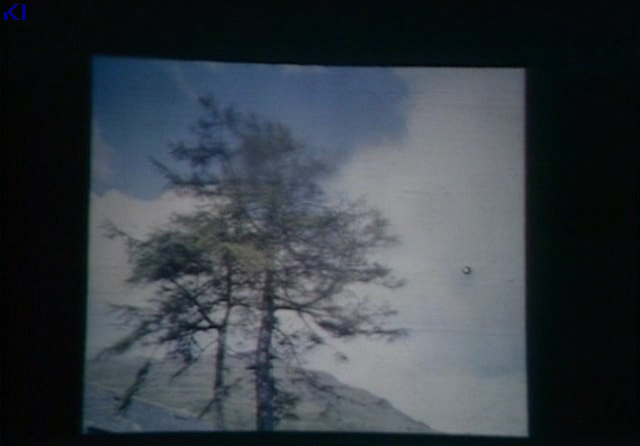
\includegraphics[width=0.8\textwidth]{larch}
  \caption{Shown is a picture of the larch as might be seen from quite a long way away.\index{Larch}}
\end{figure}

\section{And Now . . . No. 1, the Larch}
\newpage
\thispagestyle{facingcaption}
\begin{center}
\vspace*{3in}
\textbf{Figure \ref{Sideways Larch}:} Here is a caption for the Larch after you have had a wee too much to drink.

\end{center}
\newpage

\begin{figure}[hb] 
  \centering
  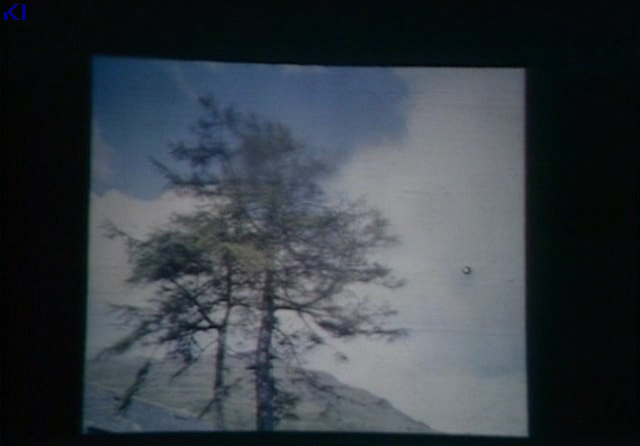
\includegraphics[width=0.8\textwidth]{larch}
  \caption[No. 1 The Larch]{Shown is a picture of the larch as might be seen from quite a long way away.\index{Larch}}\label{Sideways Larch}
\end{figure}

% Here I am testing that page breaking on the TOC works correctly.
% We never want the page break directly after a chapter entry.
\chapter{Another chapter}
\section{Some Stuff You Probably Don't Want to Read}
\section{Some Stuff You Really Don't Want to Read, it is Utterly and Completely Dull}
%\section{Now I am Just Writing Filler}
%\section{More Filler}
%\subsection{How Many Lines Am I at?}
%\subsection{Stuff}
%\section{Stuff}
%\section{Ooo-De-Laly}
%\subsection{Ooo-De-Laly, Ooo-De-Laly}
%\section{Slithy Toves}


\chapter{On the Inner Workings of a Grad Student Mind}
\section{Before Thesis Writing Has Begun}
\section{During Thesis Writing}
\section{During Thesis Formatting}
\section{After Thesis Writing}
\section{Before Defense}
\section{After Defense}

The Mock Turtle sighed deeply, and drew the back of one flapper across his eyes. He looked at Alice, and tried to speak, but for a minute or two sobs choked his voice. `Same as if he had a bone in his throat,' said the Gryphon: and it set to work shaking him and punching him in the back. At last the Mock Turtle recovered his voice, and, with tears running down his cheeks, he went on again:


\begin{verbatim}
``There's a porpoise close behind us, and he's treading on my tail.
See how eagerly the lobsters and the turtles all advance!
They are waiting on the shingle--will you come and join the dance?

Will you, won't you, 
                will you, won't you, 
                                will you join the dance?
Will you, won't you, 
                will you, won't you, 
                                won't you join the dance?''
\end{verbatim}



So Alice began telling them her adventures from the time when she first saw the White Rabbit. She was a little nervous about it just at first, the two creatures got so close to her, one on each side, and opened their eyes and mouths so very wide, but she gained courage as she went on. Her listeners were perfectly quiet till she got to the part about her repeating `You are Old, Father William,' to the Caterpillar\footnote{Which we introduced in a different thesis}, and the words all coming different, and then the Mock Turtle drew a long breath, and said `That's very curious'.

\appendix
\chapter{Final notes}
  Remove me in case of abdominal pain.





%% END MATTER
\printindex %% Uncomment to display the index
% \nocite{}  %% Put any references that you want to include in the bib 
%               but haven't cited in the braces.
% \bibliographystyle{alpha}  %% This is just my personal favorite style. 
%                              There are many others.
% \bibliography{myrefs}  %% This looks for the bibliography in myrefs.bib 
%                          which should be formatted as a bibtex file.
\end{document}

